\section*{Literature Survey}
The phenomenon of blink is at an unusual crossroad of a variety of scientific and medical disciplines, as it provides information on ocular surface health, on the cognitive state, on psychological health and disease, and on alertness and fatigue. Precisely for this reason, the blink process is difficult to study: with local and far-reaching, endogenous and exogenous input, the output is seldom driven by one overriding force.

	A blink can be defined as a lid closure of varying speed, frequency, force, and duration. The normal blink rate is about 12 blinks/minute, and the variability among individuals and with the task is widely recognized.\cite{9302890}[1]
\bibliographystyle{ieeetr}
\bibliography{citation}.The below table shows the different factors that affect the blink.
\begin{figure}[h]
    \centering
    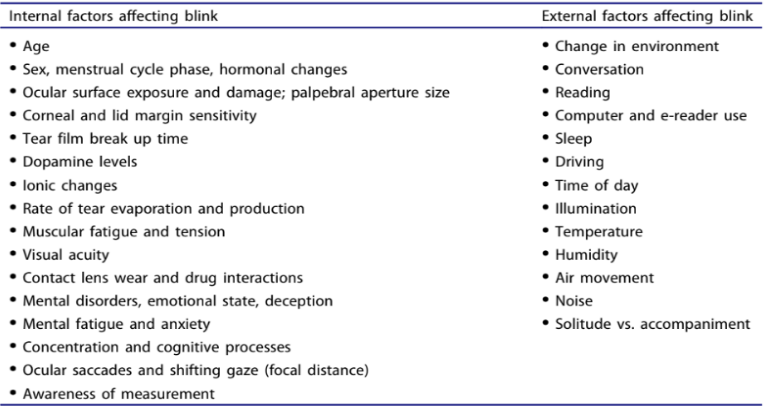
\includegraphics[height=6.5cm]{images/factors.png}
\end{figure}	
	
Our main focus is to detect eye blinks and there are various methods for the same. The two Major methods are as follows:
\begin{enumerate}
\item \textbf{Image processing: }
Image processing is a method to perform some operations on an image, to get an enhanced image, or to extract some useful information from it. It is a type of signal processing in which input is an image and output may be an image or characteristics/features associated with that image. In the paper[2], a web camera is used. Using the Viola-Jones technique face is being detected and after that eyes are detected using the thumb rule. From eyes, eye blinking was determined by converting the eyes template in binary form, which is used afterward for application.
\item \textbf{Wearable Sensors: }
\begin{itemize}
\item \textbf{Electrooculography (EOG)} - Blinks are measured with the EOG when the electrodes are placed vertically above the eyebrow and on the malar prominence in line with the pupil and it is defined as minimal voltage change during a certain period of time.[3]
\item \textbf{Electromyography (EMG)} is habitually used in blinking research to register the relationship between the orbicularis oculi muscle (OOM) and levator palpebrae superioris muscle (LPS).EMG is usually coupled to another system, such as a magnetic search coil or EOG that allows the registration of eyelid positional changes. The simultaneous use of EMG and EOG may be particularly useful for recording eyelid position OOM activity in situations where fixation of the head is not possible.[4]
\item \textbf{Infrared} reflectance utilizes an infrared (IR) LED to illuminate the eye surface and another device, such as a phototransistor or a photodiode, that detects IR light reflected back from the eye. The blink signal is analyzed based on the difference between the light emitted and the light reflected from eyelid and eyeball and is processed by a microcomputer equipped with an analog-to-digital (AD) converter.[5]
\item \textbf{Electroencephalography (EEG)} is at the core of brainwave technology. In EEG it monitors and records the brain activities with the use of electrodes that are attached to a persons’ head. Brains’ neurons emit electrical impulses to communicate with the rest of our bodies which are recorded by electrodes. In the past few years, there’s a rapid advancement and improvement which led to the development of more affordable EEG. This opened limitless possibilities in brainwave technology.[6]
\end{itemize}
\end{enumerate}

After going through all the possible methods, we finally choose to use an EEG device for this project. Because, these are non-invasive, portable, and less expensive than other devices.


\section*{Motivation}
\begin{itemize}
\item The pandemic has increased our dependence on screens for activities that could otherwise have been done offline.A new study and survey  released by NortonLifeLock, examining consumers’ at-home online behaviours, show that two in three Indians surveyed (66\%) have become addicted to being online as a result of the pandemic.The amount of time they spent on screens, aside from educational or work purposes, has increased significantly during the Covid-19 pandemic.Exposure to gadgets can have long term effects specifically when it comes to eyes.Hence using blink analysis it's possible to detect disease related to eyes at an early stage and treat it well.
\item Building an application using a wearable device to detect eye blinks which can help detect various eye-related diseases.
\item Real time analysis -  Analyzing a patient's blink data in real-time helps to identify the abnormalities in the blink rate or parameters related to blinking can help the patient get diagnosed early.
\end{itemize}

\section*{Methodology}
\begin{figure}[h]
    \centering
    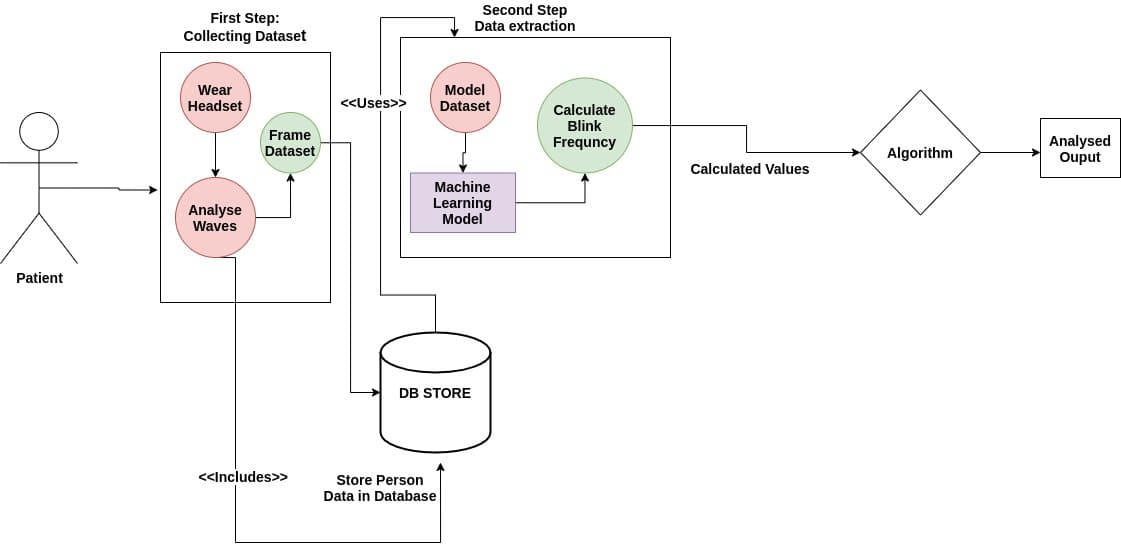
\includegraphics[height=7.5cm]{images/uml.jpg}
\end{figure}
